\documentclass[conference]{IEEEtran}

\usepackage{cite}
\usepackage{amsmath,amssymb,amsfonts}
\usepackage{algorithmic}
\usepackage{graphicx}
\usepackage{textcomp}
\usepackage{xcolor}
\usepackage{booktabs}
\usepackage{microtype}
\usepackage{url}
\usepackage{tikz}
\usepackage{pgfplots}
\pgfplotsset{compat=1.18}
\usetikzlibrary{arrows.meta, positioning, shapes.geometric, fit, backgrounds, calc}
\usepackage{subfig}
\usepackage[hidelinks]{hyperref}

\begin{document}

\title{Native Binarization: Training 1-Bit-Weight Diffusion\\Models from Scratch on MNIST}

\author{
\IEEEauthorblockN{Nihal Gazi}
\IEEEauthorblockA{Dept. CSE AI \& ML, IEM\\nihlg2006@gmail.com}
\and
\IEEEauthorblockN{Ayushman Bhattacharya}
\IEEEauthorblockA{MyceliAI A\"U\\ayushman@myceli.ai}
\and
\IEEEauthorblockN{Aditya K. Biswas}
\IEEEauthorblockA{Dept. CSE \& Business Systems, IEM\\adityakb@gmail.com}
\and
\IEEEauthorblockN{Saubhagya Kunti}
\IEEEauthorblockA{Dept. CSE \& Business Systems, IEM\\sauabhagya.kunti@gmail.com}
\and
\IEEEauthorblockN{Aihik Basu}
\IEEEauthorblockA{Dept. CSE Engineering, IEM\\aihik.basu@gmail.com}
}

\maketitle

\begin{abstract}
The memory footprint and arithmetic cost of floating-point weights are a
central obstacle to running generative diffusion models on edge hardware.
Binarizing weights to a single bit would help on both fronts, but a widely
held view---articulated most recently by the Binarized Diffusion Model
(BiDM)~\cite{bidm2024}---is that fully binarizing a diffusion network is
\emph{catastrophic}, and that recovery requires distilling from a
full-precision teacher. In this paper we revisit that claim in a deliberately
small and controlled setting: unconditional generation of $28{\times}28$ MNIST
digits. Rather than treating binarization as a post-hoc compression step, we
train a residual U-Net with 1-bit weights \emph{from random initialization}---an
approach we call \textbf{Native Binarization}---using mean-centered weight
scaling and pre-activation residual blocks. In a controlled W1A16 comparison
(binary weights with full-precision activations, so that only the binarization
\emph{methodology} varies), Post-Training Quantization (PTQ) does collapse on
this benchmark (FID~191.94, legibility~64.92\%), consistent with the
catastrophic-failure narrative, whereas the natively trained model reaches
FID~24.24 with 89.45\% legibility---comparable to an FP16 baseline of identical
architecture (FID~29.60, 90.79\%). A fully binary W1A1 variant degrades but does
not collapse (FID~83.98). We emphasize that these findings are confined to
MNIST, whose data manifold is far simpler than that of natural images; we
therefore present them not as a general solution to binary diffusion but as
preliminary evidence that, at least on this benchmark, the collapse commonly
attributed to 1-bit precision is better explained by the train-then-quantize
pipeline than by binarization itself. All code and checkpoints are released to
support replication.
\end{abstract}

\noindent\textbf{Keywords:} 1-Bit Quantization, Diffusion Models, Model Compression, Binary Neural Networks,
Post-Training Quantization, ResUNet, Edge AI, MNIST

\section{Introduction}

Denoising diffusion models have become one of the most capable families of
generative models in machine learning. Denoising Diffusion Probabilistic Models
(DDPMs)~\cite{ho2020ddpm} produce high-quality images across many domains, but
their reliance on floating-point matrix arithmetic ties them to power-hungry
GPUs and server-grade accelerators. With growing interest in on-device
intelligence---in mobile phones, wearables, and IoT sensors---this dependence is
a practical concern: executing the hundreds or thousands of sequential denoising
steps a typical DDPM requires is difficult on an edge processor today.

One appealing direction is to push weight precision toward its minimum: a single
bit. Compressing 16- or 32-bit parameters into $\{-1,+1\}$ values would replace
costly multiply--accumulate (MAC) instructions with XNOR-popcount logic, reducing
both memory and energy substantially. A recurring conclusion in the literature,
however, is that such extreme compression breaks diffusion models. The most
recent study of this question---the Binarized Diffusion Model
(BiDM)~\cite{bidm2024}, presented at NeurIPS 2024---states plainly that ``the
impact of fully binarizing weights and activations is catastrophic,'' and builds
an elaborate distillation pipeline from a full-precision teacher to recover
usable quality.

This paper is a small, focused attempt to look more closely at \emph{where} that
catastrophe comes from. Our starting observation is that binarization has, in
practice, almost always been applied as \textbf{Post-Training Quantization
(PTQ)}: a carefully trained floating-point model has its weights snapped to
binary values after the fact. This ``train first, binarize later'' pipeline
discards the finely tuned magnitude relationships that encode the learned score
field. We ask a simple question: if the weights are constrained to be binary
\emph{from the first gradient step}, rather than compressed after training, does
the collapse still occur?

We study this question in a deliberately narrow setting---unconditional MNIST
generation at $28{\times}28$ resolution---and refer to the from-scratch approach
as \textbf{Native Binarization}. It treats binarization as a problem of
\emph{representation} rather than compression: starting from random
initialization, gradient descent (via the straight-through estimator) searches
for a configuration of $\{-1,+1\}$ weights that directly minimizes the DDPM
loss. Two design choices support this: (1)~\textbf{mean-centered weight scaling},
which preserves what we informally call \emph{structural dominance}---the dominant
directional structure of each filter is retained after binarization---and
(2)~\textbf{pre-activation residual ordering} (BN\,$\to$\,Act\,$\to$\,Conv),
which we use to keep gradient flow through binary layers well-conditioned during
training (\emph{topological stability}). We frame both as working hypotheses that
are consistent with our observations, not as proven laws.

Our central comparison is a controlled \textbf{W1A16} ablation: activations are
held at full precision while only the weight-binarization method varies (PTQ
versus native). On MNIST, PTQ degrades sharply (FID~191.94,
legibility~64.92\%)---the kind of collapse the catastrophic-failure view
predicts---whereas the natively trained binary-weight model reaches FID~24.24
with 89.45\% legibility, comparable to an FP16 baseline of the same architecture
(FID~29.60, 90.79\%). We are cautious about the direction of this small gap and
do not claim the binary model is genuinely \emph{better} than full precision; we
read it as ``no meaningful loss on this benchmark.'' A fully binary W1A1 variant
(binary weights and activations) degrades to FID~83.98 but remains far from
collapse.

\textbf{Scope and contributions.} We want to be explicit that this is a
small-scale study on a single, simple dataset. MNIST digits occupy a far
lower-dimensional manifold than natural images, and results here need not
transfer to CIFAR-10, CelebA, or LSUN. Within that scope, our contributions are:
\begin{itemize}
  \item We provide preliminary evidence, on MNIST, that a 1-bit-weight diffusion
    model trained \emph{from scratch}---with no full-precision teacher, no
    distillation, and no pre-trained starting point---can match an FP16 baseline
    of identical architecture. This is a limited but concrete counterpoint to the
    view that distillation from a teacher is indispensable for binary diffusion.
  \item We articulate two informal design principles---\textbf{structural
    dominance} (centered binarization preserves directional weight geometry) and
    \textbf{topological stability} (pre-activation ordering keeps binary training
    well-conditioned)---that are consistent with why native training behaves
    differently from PTQ in our experiments.
  \item We construct a controlled \textbf{W1A16 ablation} that isolates the
    weight-binarization methodology from activation-quantization noise, enabling a
    direct PTQ-versus-native comparison at the 1-bit weight boundary on MNIST.
  \item We report a simple \textbf{Legibility Score}, a per-sample class-confidence
    metric that complements FID by measuring whether each generated digit commits
    to a recognizable class, and use it alongside FID across the FP16, W1A16, and
    W1A1 regimes.
\end{itemize}


\section{Related Work}

\subsection{Diffusion Models and Edge Deployment}

A DDPM~\cite{ho2020ddpm} corrupts training images with Gaussian noise over $T$
forward steps and trains a network $f_\theta$ to reverse this corruption, with
loss
\begin{equation}
  \mathcal{L} = \mathbb{E}_{x_0,\varepsilon,t}\!\left[
    \left\|\varepsilon - f_\theta\!\left(\sqrt{\bar\alpha_t}\,x_0 +
    \sqrt{1-\bar\alpha_t}\,\varepsilon,\;t\right)\right\|^2\right]
  \label{eq:ddpm}
\end{equation}
where $\bar\alpha_t = \prod_{i=1}^{t}(1-\beta_i)$. Follow-up work---including
DDIM~\cite{song2020ddim}, Latent Diffusion~\cite{rombach2022ldm}, and
SDXL~\cite{podell2023sdxl}---has improved image quality substantially, yet every
variant inherits the same inference bottleneck: many sequential forward passes
through the denoising network. Efforts to bring diffusion models to edge devices
have largely targeted sampling speed (e.g.\ progressive
distillation~\cite{salimans2022progressive}) or network pruning; neither
addresses the underlying cost of floating-point arithmetic itself.

\subsection{Post-Training Quantization and Its Limits}

PTQ takes an already-trained model and re-maps its floating-point parameters to a
lower bit-width without retraining. Q-Diffusion~\cite{li2023qdiffusion} and
PTQD~\cite{he2023ptqd} showed that diffusion models can be quantized to 4 or 8
bits with tolerable quality loss, and later methods added timestep-aware
calibration to account for the fact that activation statistics shift across
denoising steps. PTQ quality nonetheless degrades quickly as bit-width shrinks;
at the 1-bit extreme, quantization error dwarfs the weight magnitudes. Our own
MNIST experiments are consistent with this: a W1A16 model produced by PTQ records
FID~191.94 and 64.92\% legibility, whereas the same architecture trained natively
under binary constraints reaches FID~24.24 and 89.45\%.

\subsection{The 1-Bit Binarization Bottleneck}

In a Binary Neural Network
(BNN)~\cite{hubara2016bnn,rastegari2016xnornet}, both weights and activations are
restricted to $\{-1,+1\}$, turning multiply--accumulate arithmetic into
XNOR-popcount logic. XNOR-Net popularized per-channel scale factors
($\alpha = \text{mean}|W|$) to narrow the quantization gap, and the
Straight-Through Estimator (STE)~\cite{bengio2013ste} enabled backpropagation
through the sign function. BNNs are effective for discriminative tasks such as
image classification~\cite{liu2020reactnet,martinez2020training}, but generative
modelling---where the network must capture a full data distribution rather than
assign labels---has seen far less exploration at the binary level.

The first attempt to fully binarize a diffusion model is
BiDM~\cite{bidm2024}, which operates at W1A1 precision and reports FID~22.74 on
LSUN-Bedrooms at $256{\times}256$. BiDM combines a Timestep-friendly Binary
Structure (TBS) with Space Patched Distillation (SPD), achieving a
28.0$\times$ storage reduction and 52.7$\times$ fewer operations, and reports
that fully binarizing weights and activations without such machinery is
catastrophic. A notable dependency is that BiDM relies on a pre-trained
full-precision teacher for its distillation stage; the from-scratch approach we
study here does not. We stress that BiDM operates at a far more demanding scale
than our MNIST study, and we do not position our results as directly comparable
to theirs.

\subsection{Pre-Activation Residual Networks}

He et al.~\cite{he2016preact} showed that moving batch normalization and the
non-linearity ahead of the convolution (BN\,$\to$\,Act\,$\to$\,Conv) improves
gradient propagation in deep residual networks. For binary layers the effect is
useful for a related reason: because BatchNorm centres and scales the incoming
activations toward zero mean and unit variance, downstream sign-based operations
sit near their decision boundary, which we found kept STE gradients better behaved
across training.

\section{The Binarization Problem: Compression vs.\ Representation}

\subsection{A Hypothesis for Manifold Collapse}

Inside a trained diffusion model the denoising function $f_\theta$ implicitly
represents the score of the data distribution---the gradient
$\nabla_x \log p_t(x)$ that pulls noisy samples back toward clean data. For any
digit class this score field carves out manifold boundaries in pixel space,
encoding stroke geometry and class identity in a high-dimensional directional
structure.

PTQ replaces every floating-point weight $w_o \in \mathbb{R}$ with
$\text{sign}(w_o)\cdot\alpha$, where the scale $\alpha = \text{mean}|W|$ attempts
to compensate for lost magnitude. Because this replacement happens layer by
layer after training, with no further gradient updates, the fine-grained
magnitude ordering the network relied on is discarded. Our interpretation---which
we offer as a hypothesis consistent with the measurements below, not as a
proof---is that over the $T=1{,}000$ reverse steps this incoherence compounds and
degrades the sampled distribution, which is what we observe as the sharp FID
increase under PTQ.

\subsection{Native Binarization as a Representation Problem}

Native Binarization flips the question around. Instead of squeezing a
floating-point solution into binary constraints, we let the network \emph{find} a
binary solution from scratch. Starting from random initialization, gradient
descent via the STE searches for a configuration of $\{-1,+1\}$ weights that
directly minimizes the DDPM noise-prediction loss. The weights that emerge are not
a degraded copy of a floating-point original; they are a binary encoding of the
score field, expressed in a different representational geometry.

Our working hypothesis is that such a natively binary solution both exists and is
reachable through standard gradient-based optimization on MNIST, given two
conditions: (1)~each binarization step preserves enough directional information to
sustain a useful gradient signal (\emph{structural dominance}), and (2)~the
gradient path through binary layers stays well-conditioned throughout training
(\emph{topological stability}). We do not claim these conditions are sufficient in
general---only that they are consistent with what we observe here.


\section{Methodology}

\subsection{Native 1-Bit Diffusion Architecture}

The backbone is a compact residual U-Net~\cite{ronneberger2015unet} with three
channel widths---$[64, 128, 256]$---and two rounds of spatial down-sampling
(MaxPool2d, $\times2$) followed by matching up-sampling stages
(nearest-neighbour, $\times2$). Encoder feature maps are concatenated with their
decoder counterparts via skip connections at every resolution. All experiments
target $28{\times}28$ single-channel MNIST~\cite{lecun1998mnist} images; the
topology is shown in Figure~\ref{fig:arch}.

\begin{figure}[t]
\centering
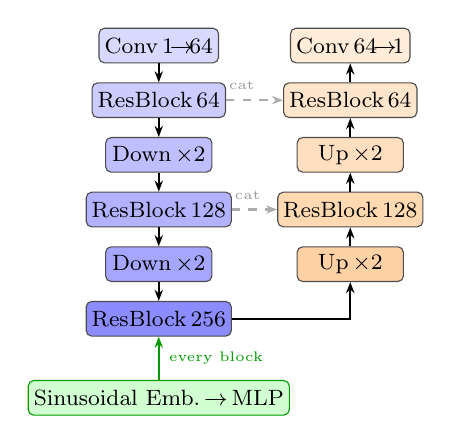
\begin{tikzpicture}[
    font=\footnotesize,
    block/.style={rectangle, rounded corners=2pt, draw=black!70,
                  fill=#1, minimum width=1.35cm, minimum height=0.44cm,
                  text centered, inner sep=2pt},
    temb/.style={rectangle, rounded corners=2pt, draw=green!60!black,
                 fill=green!18, minimum width=2.9cm, minimum height=0.44cm,
                 text centered, inner sep=2pt},
    arr/.style={-{Stealth[length=4pt]}, thick},
    skip/.style={-{Stealth[length=4pt]}, dashed, gray!65, thick},
    garr/.style={-{Stealth[length=4pt]}, green!60!black, thick},
    node distance=0.24cm and 0.9cm
  ]


  \node[block=blue!15]                   (in)  {Conv\,1$\!\to\!$64};
  \node[block=blue!20, below=of in]      (e1)  {ResBlock\,64};
  \node[block=blue!25, below=of e1]      (d1)  {Down\,$\times$2};
  \node[block=blue!30, below=of d1]      (e2)  {ResBlock\,128};
  \node[block=blue!35, below=of e2]      (d2)  {Down\,$\times$2};
  \node[block=blue!45, below=of d2]      (bot) {ResBlock\,256};

  \node[block=orange!15, right=0.9cm of in]  (out) {Conv\,64$\!\to\!$1};
  \node[block=orange!20, below=of out]       (de1) {ResBlock\,64};
  \node[block=orange!25, below=of de1]       (u1)  {Up\,$\times$2};
  \node[block=orange!30, below=of u1]        (de2) {ResBlock\,128};
  \node[block=orange!35, below=of de2]       (u2)  {Up\,$\times$2};


  \node[temb, below=0.55cm of bot] (te)
        {Sinusoidal Emb.\,$\to$\,MLP};

  \foreach \a/\b in {in/e1, e1/d1, d1/e2, e2/d2, d2/bot}
    \draw[arr] (\a) -- (\b);

  \draw[arr] (bot.east) -| (u2.south);

  \foreach \a/\b in {u2/de2, de2/u1, u1/de1, de1/out}
    \draw[arr] (\a) -- (\b);

  \draw[skip] (e1.east)  -| ++(0.2, 0) |- (de1.west)
        node[pos=0.25, above, gray!80, font=\tiny]{cat};
  \draw[skip] (e2.east)  -| ++(0.2, 0) |- (de2.west)
        node[pos=0.25, above, gray!80, font=\tiny]{cat};

  \draw[garr] (te.north) -- (bot.south)
        node[midway, right, font=\tiny, green!60!black]{every block};

\end{tikzpicture}
\caption{Residual U-Net architecture shared across all three model variants (FP16,
W1A16, W1A1). The encoder--decoder structure with channel widths [64,~128,~256],
skip connections (dashed, via concatenation), and sinusoidal time embedding
injection (green) is identical in all variants; only the convolution type changes
(Conv2d / BitConv2d\_Std / BitConv2d\_BNN).}
\label{fig:arch}
\end{figure}

\textbf{Time Conditioning.} Each diffusion step index is encoded with a
32-dimensional sinusoidal embedding~\cite{vaswani2017attention} and fed through a
small two-layer MLP, producing $t_\text{emb} \in \mathbb{R}^{32}$. Inside every
residual block a learned linear layer maps $t_\text{emb}$ to the block's channel
count and adds it element-wise to the feature map, so timestep information is
available at all spatial resolutions.

\textbf{Boundary Layer Convention.} Following standard BNN practice, the input
convolution ($1{\to}64$) and the output projection ($64{\to}1$) remain in full
precision across all variants. Keeping the pixel-space interface layers at higher
precision avoids introducing quantization noise at the boundaries of the network.

\subsection{Pre-Activation Block Structure}

Every binary residual block follows the pre-activation layout in
Figure~\ref{fig:block}. A single block computes:
\begin{align*}
  h &\leftarrow \text{BinaryAct}\!\left(\text{BN}(x)\right) \\
  h &\leftarrow \text{BinaryConv2d}(h) \\
  h &\leftarrow h + \text{Linear}(t_\text{emb}) \\
  h &\leftarrow \text{BinaryAct}\!\left(\text{BN}(h)\right) \\
  h &\leftarrow \text{BinaryConv2d}(h) \\
  \text{output} &\leftarrow h + \text{skip}(x)
\end{align*}
where \texttt{skip} is a 1$\times$1 binary convolution when channel dimensions
change and an identity otherwise. In the W1A16 variant, \texttt{BinaryAct} is a
full-precision activation (SiLU) and only the weights are binarized; in the W1A1
variant, \texttt{BinaryAct} is the clipped-STE sign activation described in
Section~\ref{sec:ste}.

\begin{figure}[t]
\centering

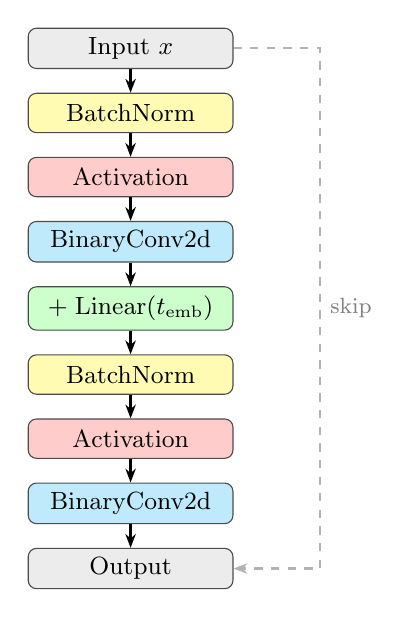
\begin{tikzpicture}[
    font=\small,
    op/.style={rectangle, rounded corners=3pt, draw=black!70,
               fill=#1, minimum width=2.6cm, minimum height=0.5cm,
               text centered},
    arr/.style={-{Stealth[length=5pt]}, thick},
    skip/.style={-{Stealth[length=5pt]}, dashed, gray!60, thick},
    node distance=0.3cm
  ]

  \node[op=gray!15]   (x)   {Input $x$};
  \node[op=yellow!30, below=of x]  (bn1) {BatchNorm};
  \node[op=red!20,    below=of bn1](ba1) {Activation};
  \node[op=cyan!25,   below=of ba1](bc1) {BinaryConv2d};
  \node[op=green!20,  below=of bc1](te)  {$+\;\text{Linear}(t_\text{emb})$};
  \node[op=yellow!30, below=of te] (bn2) {BatchNorm};
  \node[op=red!20,    below=of bn2](ba2) {Activation};
  \node[op=cyan!25,   below=of ba2](bc2) {BinaryConv2d};
  \node[op=gray!15,   below=of bc2](out) {Output};

  \foreach \a/\b in {x/bn1, bn1/ba1, ba1/bc1, bc1/te,
                     te/bn2, bn2/ba2, ba2/bc2, bc2/out}
    \draw[arr] (\a) -- (\b);

  \draw[skip] (x.east) -- ++(1.1,0) |- (out.east)
    node[pos=0.25, right, font=\footnotesize, gray]{skip};

\end{tikzpicture}
\caption{Pre-activation binary residual block. BatchNorm is applied \emph{before}
the activation at both sub-layers, keeping the inputs to downstream binary
operations approximately zero-centred during training (topological stability). The
identity skip connection preserves gradient flow to shallow layers. The activation
is SiLU for W1A16 (weights binarized only) and the clipped-STE sign function for
W1A1 (weights and activations binarized).}
\label{fig:block}
\end{figure}

\textbf{Topological Stability via Pre-Activation Ordering.} The motivation for
this ordering is that BatchNorm re-centres and re-scales activations
\emph{before} they reach the following operation. Because the resulting
distribution sits near zero mean with unit variance, sign-based operations stay
close to their decision boundary during training. In our runs this ordering
avoided the dead-neuron and gradient-starvation behaviour we observed with other
orderings. We use \textbf{topological stability} as an informal name for this
property: the binary representation stays balanced enough to keep training stable
and to capture the class-level structure of the data on this benchmark.

\subsection{Mean-Centered Weight Binarization (Structural Dominance)}

Weight binarization in the W1A16 variant is handled by \texttt{BitConv2d\_Std}, a
convolution layer that subtracts the per-filter mean before applying the sign
function. Given a weight tensor $W \in \mathbb{R}^{C_\text{out} \times C_\text{in}
\times k \times k}$, let $w_o \in \mathbb{R}^{C_\text{in}k^2}$ denote the
flattened kernel for output channel $o$.

\textbf{Standard (uncentered) binarization:}
\begin{equation}
  \tilde{w}_o = \operatorname{sign}(w_o)\cdot\alpha_o,
  \quad
  \alpha_o = \frac{\|w_o\|_1}{C_\text{in}\cdot k^2}
  \label{eq:std-bin}
\end{equation}

\textbf{Centered binarization (\texttt{BitConv2d\_Std}):}
\begin{equation}
  \bar{w}_o = w_o - \mu_o,
  \quad
  \mu_o = \operatorname{mean}(w_o)
  \label{eq:center}
\end{equation}
\begin{equation}
  \hat{w}_o = \operatorname{sign}(\bar{w}_o)\cdot\bar\alpha_o,
  \quad
  \bar\alpha_o = \frac{\|\bar{w}_o\|_1}{C_\text{in}\cdot k^2}
  \label{eq:cen-bin}
\end{equation}

\textbf{Structural Dominance Property.} By subtracting $\mu_o$, the isotropic DC
component is removed from the weight vector, leaving its directional content. The
sign function then quantizes this centred direction, while $\bar\alpha_o$ serves
as a magnitude proxy that rescales the result. The intended effect is that
$\hat{w}_o$ retains the \emph{dominant directional structure} of the original
filter $w_o$: a zero-mean vector's sign pattern reflects how its entries are
distributed across directions more faithfully than that of a vector biased by a
large DC offset, so centering reduces the angular distortion that binarization
introduces. We expect this to matter for diffusion networks, whose convolutional
kernels must capture oriented denoising responses to approximate the score field.

\subsection{Gradient Approximation via Straight-Through Estimator}
\label{sec:ste}

Both weight and activation binarization rely on the sign function, which has zero
derivative almost everywhere. To enable backpropagation through this hard
threshold we use the \textbf{Straight-Through Estimator}
(STE)~\cite{bengio2013ste}.

\textbf{Weight STE (\texttt{BitConv2d\_Std} and \texttt{BitConv2d\_BNN}):}
\begin{equation}
  w_\text{forward} = \underbrace{(\hat{w}_o - w_o)}_{\text{stop-grad}} + w_o
  \label{eq:ste-w}
\end{equation}

\textbf{Activation STE (W1A1 only, clipped):}
\begin{equation}
  \text{BinaryAct}(x) = \operatorname{sign}(x),
  \quad
  \frac{\partial\,\text{BinaryAct}}{\partial x} = \mathbf{1}[|x|\le 1]
  \label{eq:ste-a}
\end{equation}

Under the clipped variant~\cite{courbariaux2016clippedste}, gradients are set to
zero whenever $|x|>1$, which suppresses the influence of outlier activations while
keeping gradient information flowing through the bulk of the distribution.

\section{Experimental Setup}

\subsection{Model Architectures and Initialization}

Three model variants, all built on an identical U-Net backbone, are evaluated.
Their configurations are summarized in Table~\ref{tab:variants}.

\begin{table}[h]
\centering
\caption{Model Variants}
\label{tab:variants}
\footnotesize
\begin{tabular}{@{}llll@{}}
\toprule
\textbf{Variant} & \textbf{Weights} & \textbf{Acts.} & \textbf{Key Layer} \\
\midrule
ResUNet\_FP16  & FP16              & FP16 (SiLU)        & Conv2d \\
ResUNet\_W1A16 & 1-bit, centered   & FP16 (SiLU)        & BitConv2d\_Std \\
ResUNet\_W1A1  & 1-bit, uncentered & 1-bit (clip.\ STE) & BitConv2d\_BNN \\
\bottomrule
\end{tabular}
\end{table}

Every model starts from PyTorch's default initialization. We train with the
standard DDPM objective under a linear noise schedule
$\beta \in [10^{-4},\,0.02]$ spanning $T=1{,}000$ diffusion steps. The FP16 and
W1A16 variants use Adam (lr $=10^{-3}$); W1A1 uses
AdamW~\cite{loshchilov2019adamw} (lr $=10^{-4}$). All variants are trained on the
full MNIST~\cite{lecun1998mnist} training split (60{,}000 images,
$28{\times}28$ grayscale, normalized to $[-1,1]$). The time-embedding MLP uses
ReLU for FP16 and W1A16 and GELU for W1A1. To reduce sampling variance, every
reported metric is averaged over three independent evaluation runs (fresh sample
draws) of the same trained checkpoint.

\subsection{The W1A16 Isolation Strategy}

Central to our design is a \textbf{controlled ablation} in which activation
precision is held fixed at FP16 and only the weight-binarization strategy differs.
This decouples the binarization methodology (PTQ versus native) from confounds
introduced by activation-quantization noise. The two variants compared are:

\begin{itemize}
  \item \textbf{ResUNet\_W1A16 (Native):} Trained from scratch with
    \texttt{BitConv2d\_Std}.
  \item \textbf{ResUNet\_W1A16 (PTQ):} The trained FP16 model with weights
    post-hoc binarized via \texttt{BitConv2d\_Std}. Biases and BatchNorm
    statistics are preserved; only the convolutional weights are binarized.
\end{itemize}

Because activation precision is identical in both settings, any gap in generation
quality can be attributed to the training methodology---native versus
post-training binarization---rather than to differences in activation
representation.

\subsection{Evaluation Metrics}

\textbf{Fr\'echet Inception Distance (FID).} We use FID~\cite{heusel2017fid},
which measures the distance between two multivariate Gaussians fit to InceptionV3
features---one from $N=2{,}000$ generated samples, the other from the MNIST test
set. Before feature extraction, all images are bilinearly upsampled from
$28{\times}28$ to $299{\times}299$ and replicated across 3 channels:
\begin{equation}
  \text{FID} = \|\mu_r - \mu_g\|^2 +
  \operatorname{Tr}\!\left(\Sigma_r + \Sigma_g -
  2(\Sigma_r\Sigma_g)^{1/2}\right)
  \label{eq:fid}
\end{equation}
We note that FID computed on MNIST with an ImageNet-trained InceptionV3 backbone
is an imperfect proxy---the feature extractor was not trained on digits---so we
treat FID here as a relative comparison across our own variants rather than an
absolute quality figure.

\textbf{Legibility Score.} As a complementary, task-specific probe we report the
Legibility Score: the average peak softmax confidence over $N=1{,}000$ generated
images, evaluated by a small MNIST classifier trained separately on real data:
\begin{equation}
  \text{Legibility} = \frac{1}{N}\sum_{i=1}^{N}
  \max_{k\in\{0,\ldots,9\}} P\!\left(k \mid x_i^{\text{gen}}\right)
  \label{eq:legibility}
\end{equation}
Values close to 1.0 indicate that generated digits commit strongly to a class;
values near 0.10 (uniform chance) indicate near-collapse.

\section{Results and Analysis}

\subsection{Quantitative Comparison}

The main results from the W1A16 ablation, together with the W1A1 variants, appear
in Table~\ref{tab:main}.

\begin{table}[h]
\centering
\caption{MNIST Benchmark: Native vs.\ Post-Training Quantization}
\label{tab:main}
\begin{tabular}{@{}llcc@{}}
\toprule
\textbf{Model} & \textbf{Strategy} & \textbf{FID~$\downarrow$} &
\textbf{Legibility~$\uparrow$} \\
\midrule
ResUNet\_FP16  & Native (baseline) & $29.60 \pm 0.23$  & $90.79 \pm 0.51$\% \\
ResUNet\_W1A16 & \textbf{Native (ours)} & $\mathbf{24.24 \pm 1.15}$  & $\mathbf{89.45 \pm 0.73}$\% \\
ResUNet\_W1A16 & PTQ               & $191.94 \pm 1.37$ & $64.92 \pm 1.16$\% \\
\midrule
ResUNet\_W1A1  & \textbf{Native (ours)} & $\mathbf{83.98 \pm 1.66}$  & $\mathbf{81.02 \pm 0.54}$\% \\
ResUNet\_W1A1  & PTQ               & $223.00 \pm 1.89$ & $63.04 \pm 0.74$\% \\
\bottomrule
\end{tabular}
\end{table}

The pattern is consistent across metrics. With native training, the W1A16 model
records FID~24.24 and legibility~89.45\%, on par with the FP16 baseline (FID~29.60,
legibility~90.79\%). We deliberately avoid reading the small FID difference as
evidence that the binary model is \emph{superior}---given the single dataset, the
imperfect FID proxy discussed above, and run-to-run variance, the honest summary
is that native binary-weight training incurs no meaningful quality loss on MNIST.
PTQ, by contrast, degrades sharply: FID~191.94 (roughly $7.9\times$ the native
model) with legibility falling to 64.92\%, consistent with the view that
retroactive binarization disrupts the learned score field, though some residual
structure clearly persists. In the fully binary W1A1 regime, native training
reaches FID~83.98 and 81.02\% legibility---markedly worse than W1A16 but far from
collapse---whereas PTQ decays further to FID~223.00 and 63.04\%. The W1A16
contrast is visualised in Figure~\ref{fig:chart}.

\begin{figure}[h]
\centering
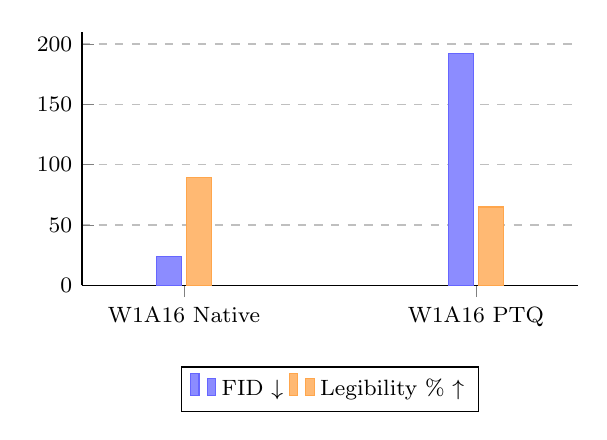
\begin{tikzpicture}
\begin{axis}[
    ybar,
    bar width=9pt,
    width=0.65\columnwidth,
    height=4.8cm,
    enlarge x limits=0.35,
    symbolic x coords={W1A16 Native, W1A16 PTQ},
    xtick=data,
    x tick label style={font=\footnotesize, align=center},
    ymin=0, ymax=210,
    ylabel style={font=\footnotesize},
    tick label style={font=\footnotesize},
    legend style={font=\footnotesize, at={(0.5,-0.32)}, anchor=north,
                  legend columns=2},
    axis y line*=left,
    axis x line*=bottom,
    ymajorgrids=true,
    grid style=dashed,
    clip=false,
    title style={font=\footnotesize\bfseries},
]

\addplot[fill=blue!45, draw=blue!60]
  coordinates {(W1A16 Native, 24.24) (W1A16 PTQ, 191.94)};
\addlegendentry{FID $\downarrow$};


\addplot[fill=orange!55, draw=orange!70]
  coordinates {(W1A16 Native, 89.45) (W1A16 PTQ, 64.92)};
\addlegendentry{Legibility \% $\uparrow$};
\end{axis}
\end{tikzpicture}
\caption{FID (lower is better, blue) and Legibility \% (higher is better, orange)
for the two W1A16 strategies on MNIST. The native model attains markedly lower FID
(24.24 vs.\ 191.94) and higher legibility (89.45\% vs.\ 64.92\%) than PTQ. Values
are means over three evaluation runs.}
\label{fig:chart}
\end{figure}

\subsection{Visual Evidence}

Figures~\ref{fig:fp16}--\ref{fig:compare3way} provide visual corroboration of the
numbers.

\begin{figure}[t]
  \centering
  \subfloat{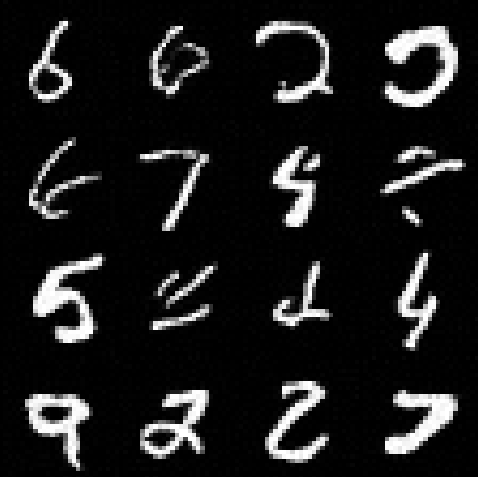
\includegraphics[width=0.35\columnwidth]{../../experiments/v0_mnist/assets/fp16_1.png}}\hfill
  \subfloat{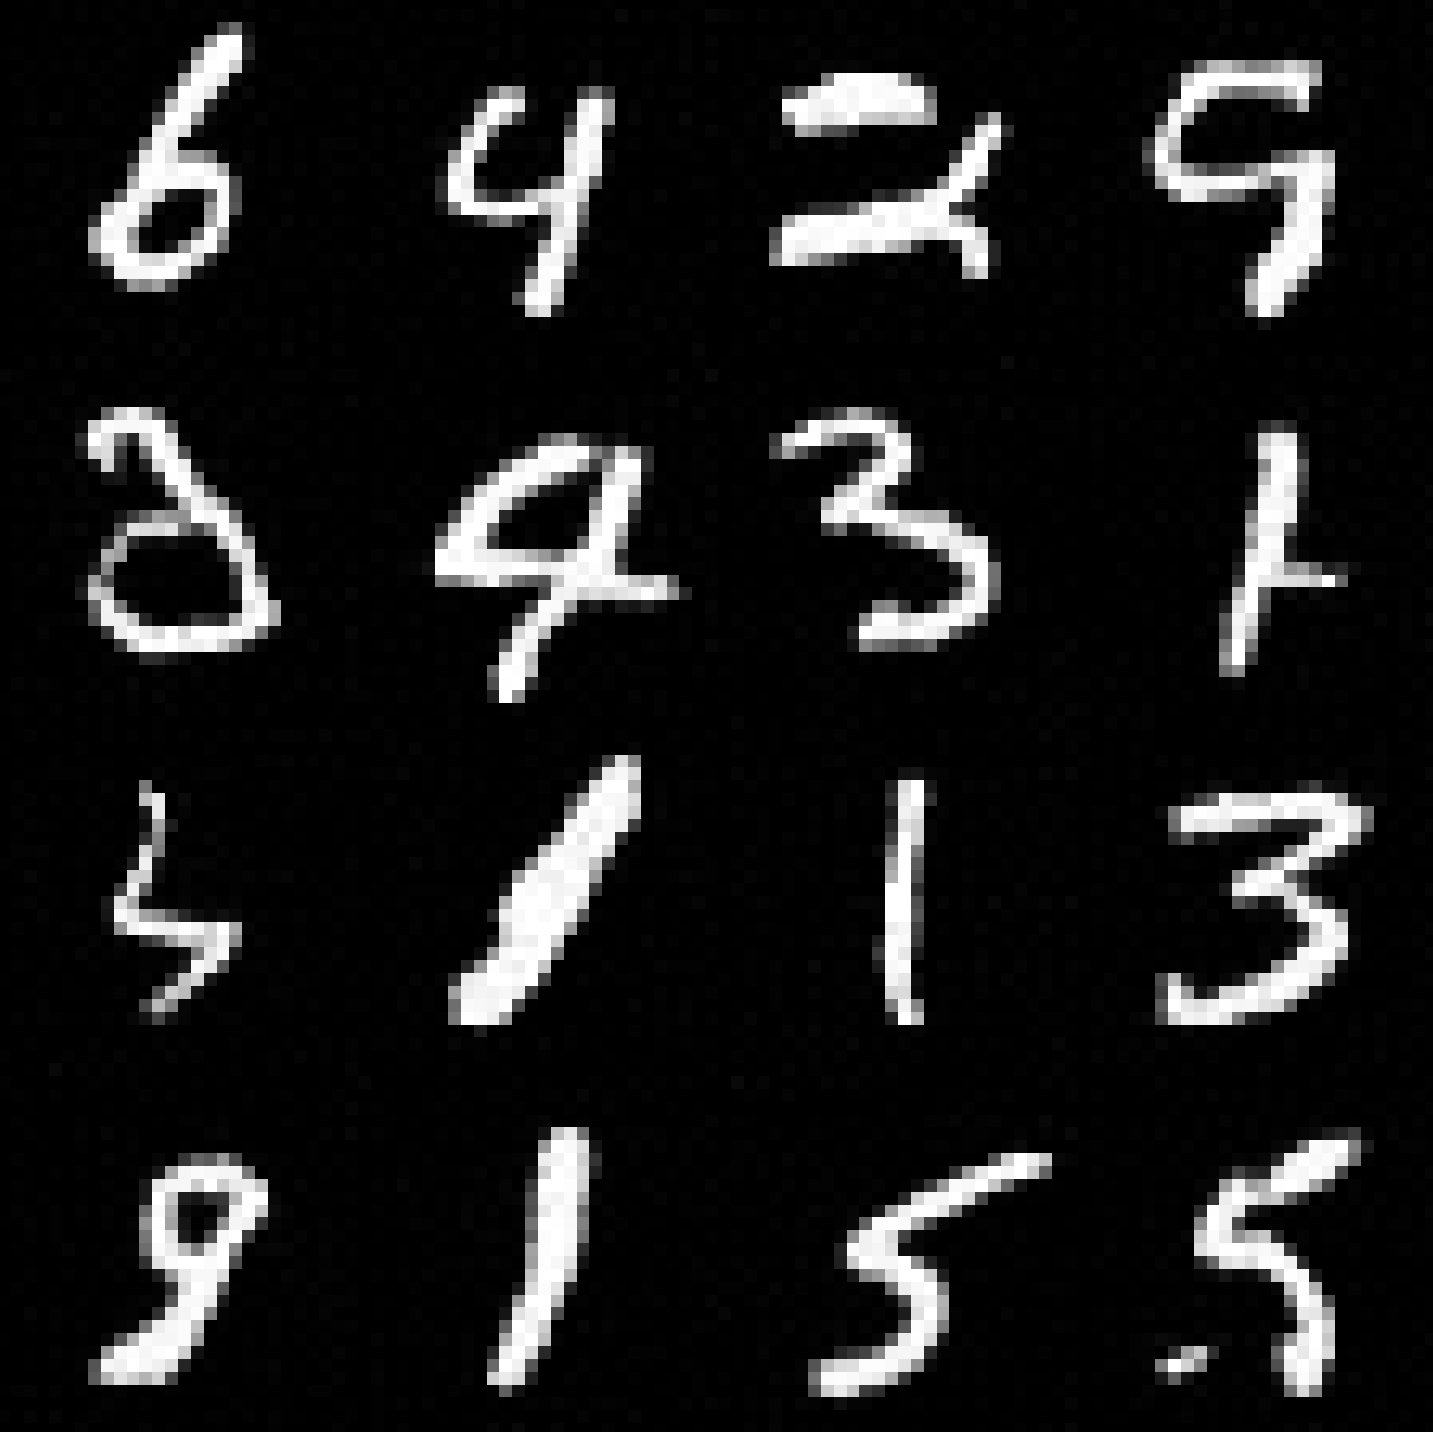
\includegraphics[width=0.35\columnwidth]{../../experiments/v0_mnist/assets/fp16_2.png}}
  \caption{ResUNet\_FP16 (full-precision baseline). Generated digits are crisp,
  varied, and clearly committed to individual classes---the quality reference for
  the compressed variants.}
  \label{fig:fp16}
\end{figure}

\begin{figure}[t]
  \centering
  \subfloat{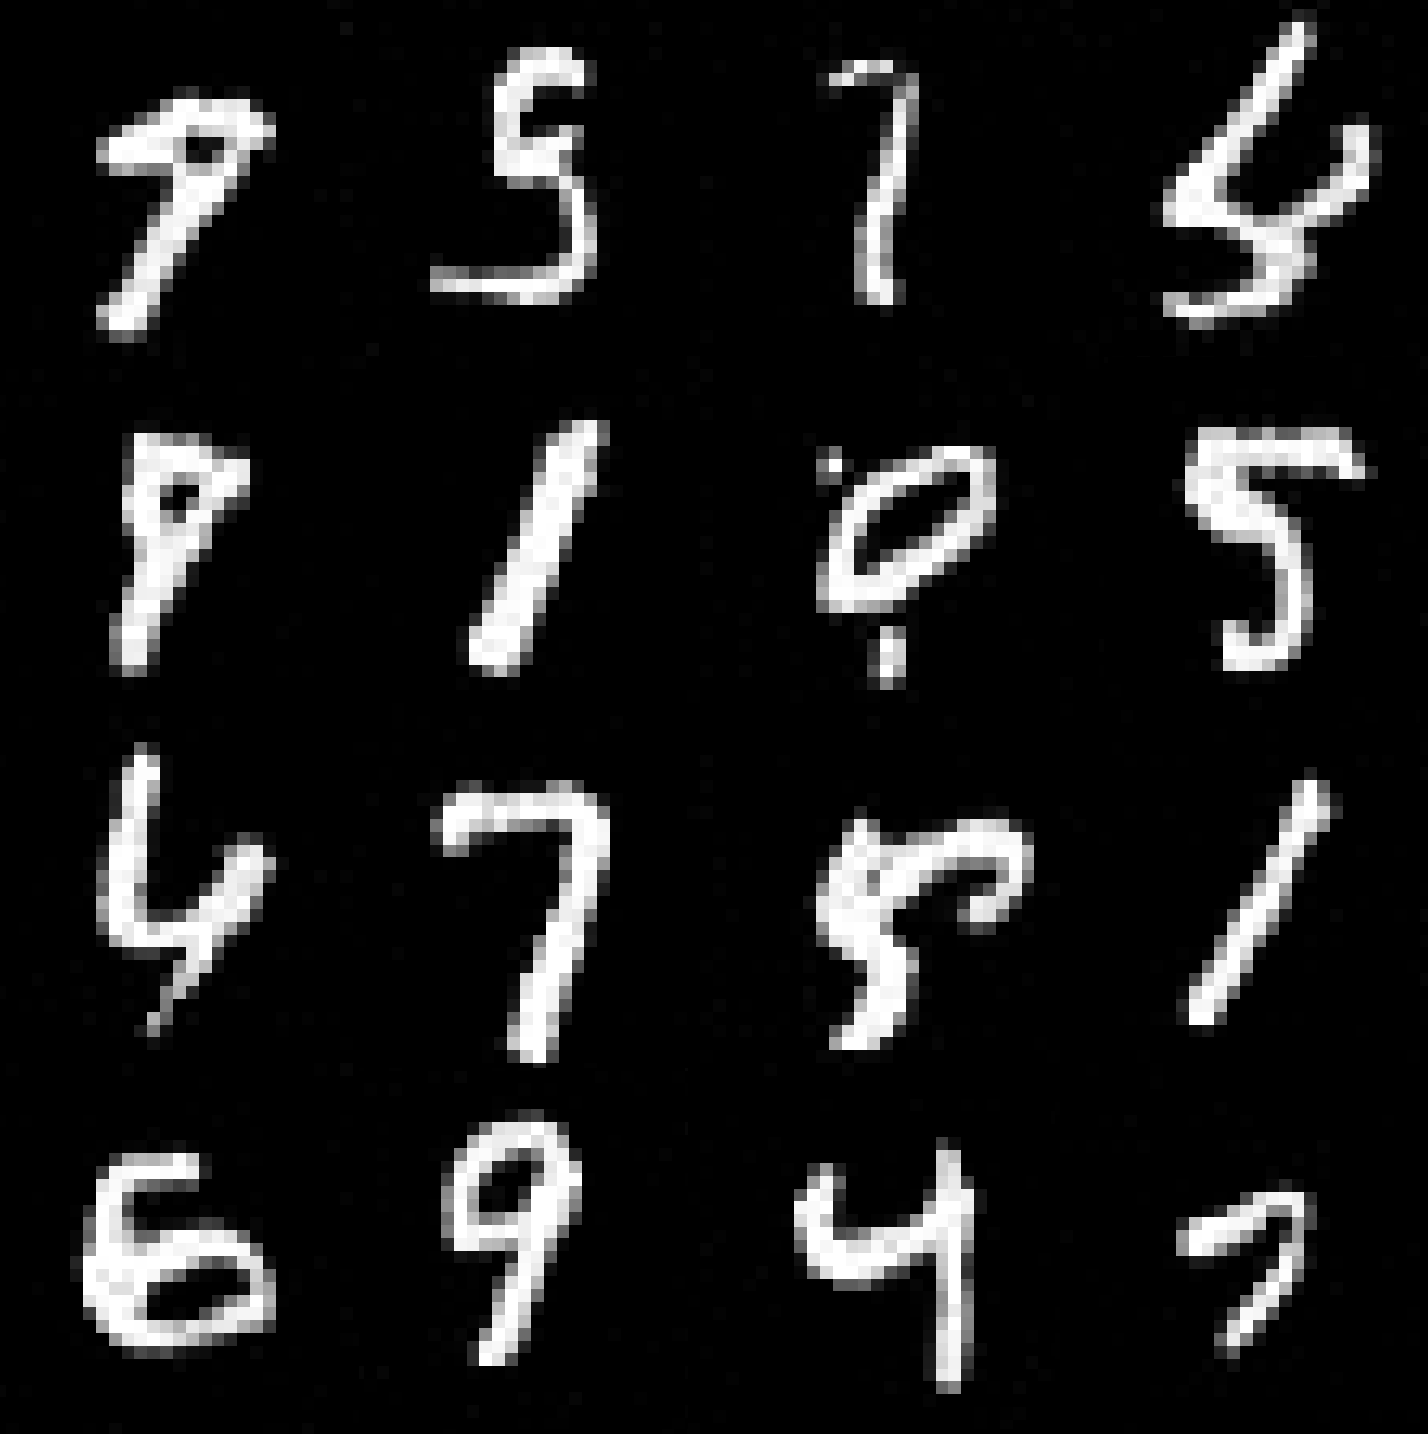
\includegraphics[width=0.35\columnwidth]{../../experiments/v0_mnist/assets/w1a16_our_output_1.png}}\hfill
  \subfloat{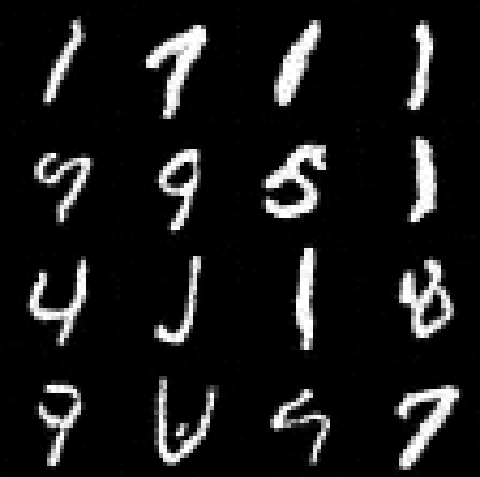
\includegraphics[width=0.35\columnwidth]{../../experiments/v0_mnist/assets/w1a16_our_output_2.png}}
  \caption{Natively trained ResUNet\_W1A16 (centered 1-bit weights, FP16
  activations). Digit structure and class diversity remain visually intact,
  consistent with the measured FID of 24.24 and 89.45\% legibility.}
  \label{fig:w1a16nat}
\end{figure}

\begin{figure}[t]
  \centering
  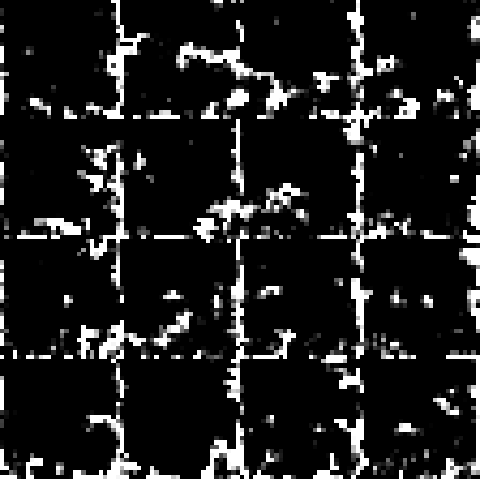
\includegraphics[width=0.45\columnwidth]{../../experiments/v0_mnist/assets/w1a16_quantized_1.png}
  \caption{PTQ ResUNet\_W1A16 (FP16 model binarized after training). Outputs show
  pronounced structural degradation, matching the measured FID of 191.94 and
  64.92\% legibility, though some residual digit structure persists.}
  \label{fig:w1a16ptq}
\end{figure}

\begin{figure}[t]
  \centering
  \subfloat{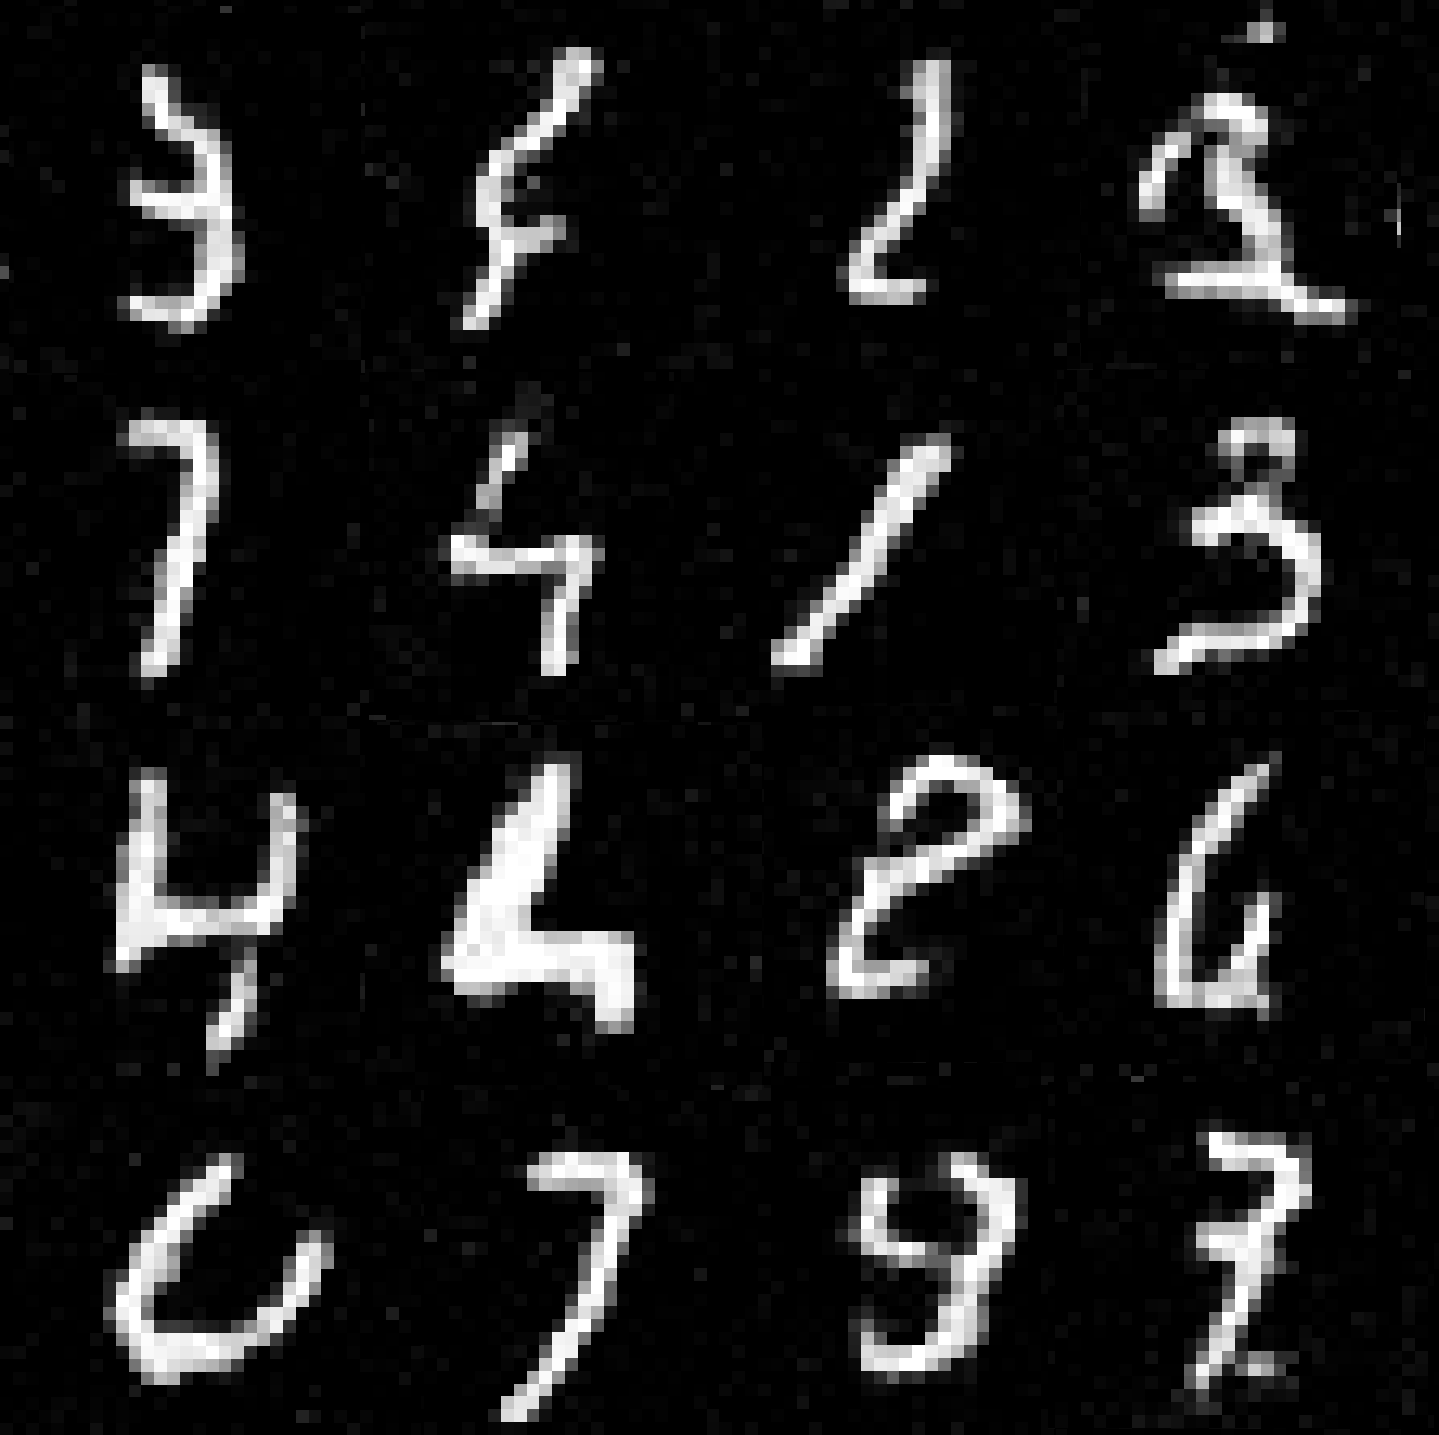
\includegraphics[width=0.35\columnwidth]{../../experiments/v0_mnist/assets/w1a1_our_output_1.png}}\hfill
  \subfloat{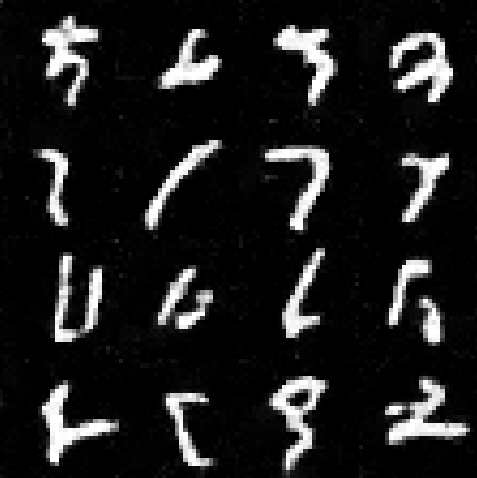
\includegraphics[width=0.35\columnwidth]{../../experiments/v0_mnist/assets/w1a1_our_output_2.png}}
  \caption{Natively trained ResUNet\_W1A1 (fully 1-bit: binary weights and
  activations, pre-activation ordering with clipped STE). Digit topology is largely
  preserved despite all-binary computation, though samples are visibly softer than
  the W1A16 model.}
  \label{fig:w1a1nat}
\end{figure}

\begin{figure}[t]
  \centering
  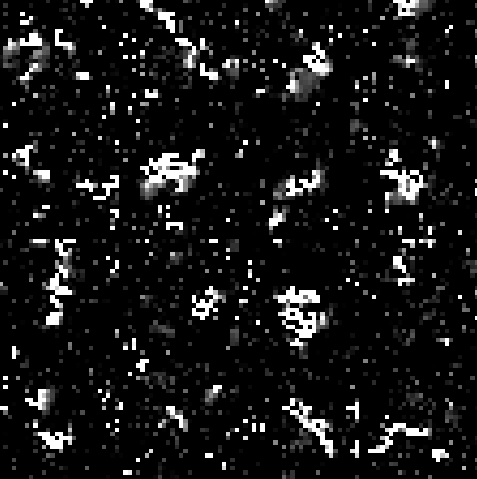
\includegraphics[width=0.45\columnwidth]{../../experiments/v0_mnist/assets/w1a1_quantized_1.png}
  \caption{PTQ ResUNet\_W1A1 (FP16 model fully binarized in both weights and
  activations). Activation binarization compounds the weight-quantization error,
  producing further degradation beyond PTQ W1A16 (Fig.~\ref{fig:w1a16ptq}).}
  \label{fig:w1a1ptq}
\end{figure}

\begin{figure}[t]
  \centering
  \subfloat[FP16]{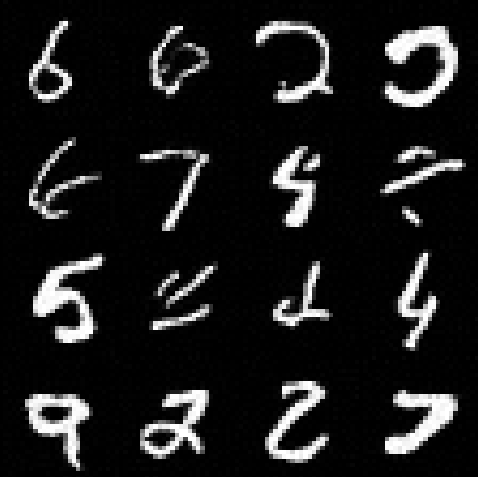
\includegraphics[width=0.22\columnwidth]{../../experiments/v0_mnist/assets/fp16_1.png}}\hfill
  \subfloat[W1A16 Native]{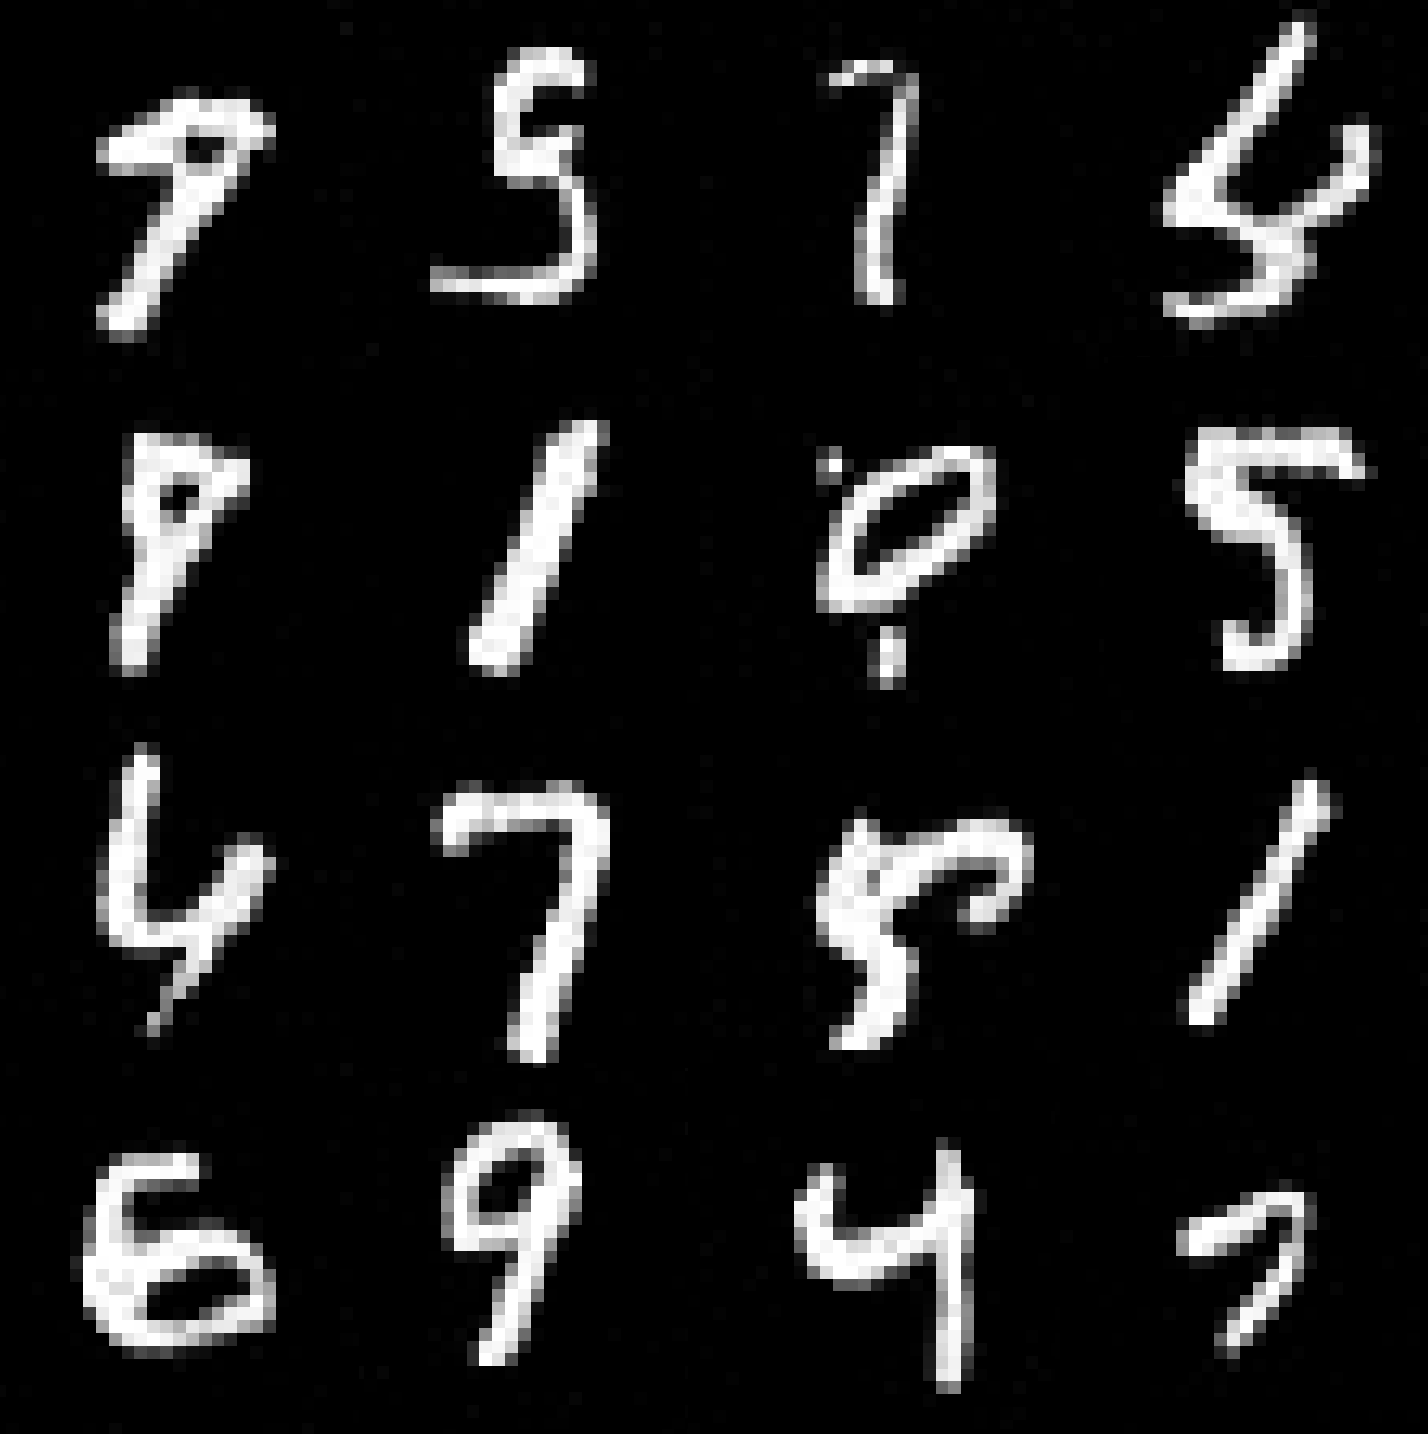
\includegraphics[width=0.22\columnwidth]{../../experiments/v0_mnist/assets/w1a16_our_output_1.png}}\hfill
  \subfloat[W1A1 Native]{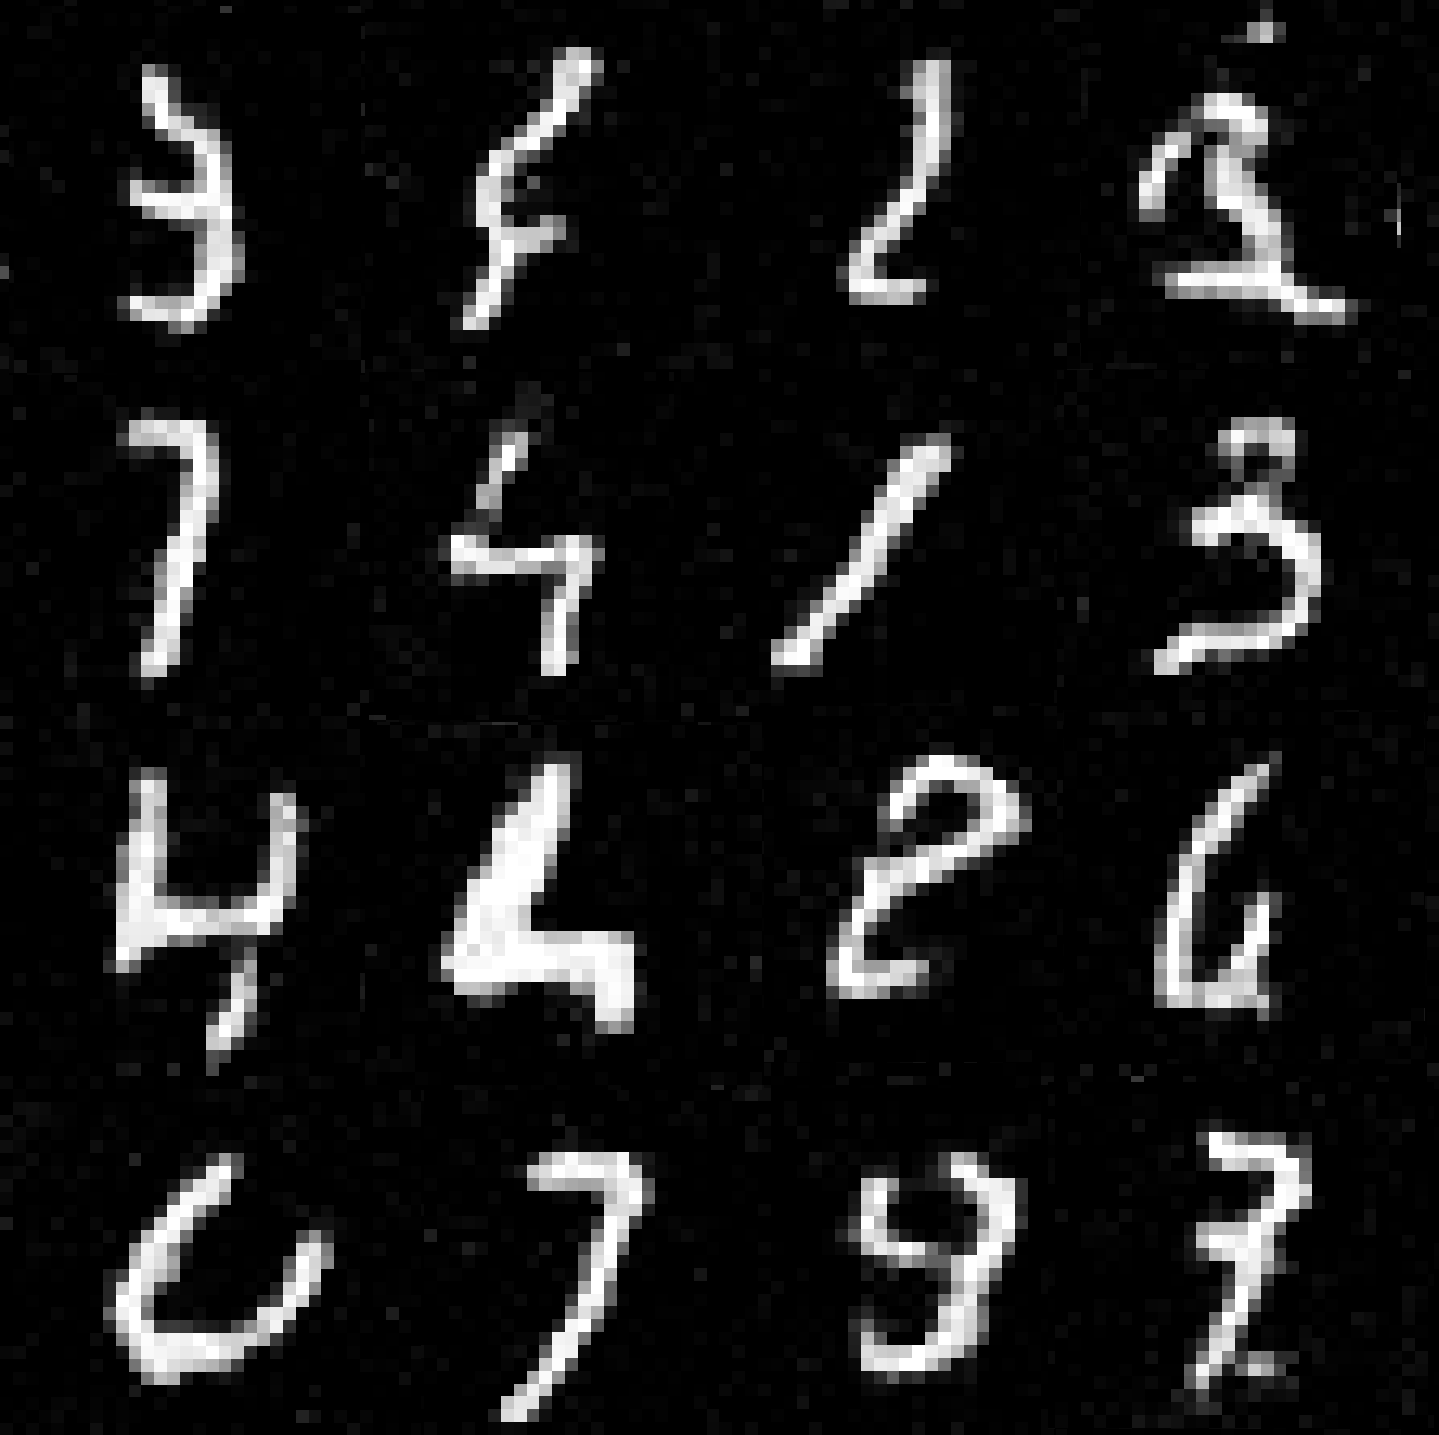
\includegraphics[width=0.22\columnwidth]{../../experiments/v0_mnist/assets/w1a1_our_output_1.png}}
  \caption{Three-way visual comparison. Quality degrades progressively with deeper
  quantization: the W1A16 native model preserves near-baseline fidelity, while W1A1
  native shows the characteristic softening expected from fully binary activations.}
  \label{fig:compare3way}
\end{figure}

\subsection{Hardware Efficiency (Theoretical)}

Relative to ResUNet\_FP16, the W1A16 model offers the following theoretical
hardware advantages. We label these as theoretical because our current
implementation uses standard PyTorch convolutions on binary-valued weight tensors
and does not yet include specialised binary kernels.

\begin{itemize}
  \item \textbf{Memory:} Each binarized convolutional weight requires only 1~bit
    versus 32~bits under FP32 storage---a \textbf{32$\times$ reduction} across the
    binarized layers (16$\times$ relative to FP16 inference weights).
  \item \textbf{Arithmetic:} Multiplication with a binary weight reduces to a sign
    flip, implementable as XNOR-popcount---a \textbf{58$\times$ reduction in binary
    operations} against the FP16 MAC count (BOPs vs.\ FLOPs).
  \item \textbf{Energy:} On dedicated binary-arithmetic hardware, such operations
    can draw roughly 1--2 orders of magnitude less energy than floating-point
    equivalents.
\end{itemize}

On MNIST these savings come at little measurable cost to class-level semantic
quality: with 89.45\% legibility versus 90.79\% for FP16, the W1A16 model produces
digits that are, at the class level, close to those of the full-precision
baseline.

\section{Discussion}

\subsection{Why PTQ Fails at 1-Bit (on This Benchmark)}

The structural-dominance view suggests a mechanism for why PTQ collapses at the
1-bit boundary. In a trained FP16 diffusion model, the score function is encoded
through the joint magnitudes and signs of filter weights. Binarization discards
the magnitude ordering and keeps only the signs; in a converged FP16 network,
individual signs carry little standalone semantic content, so extracting them
post-hoc removes most of the encoding.

A complementary explanation is landscape-theoretic. The loss surfaces of the DDPM
objective under binary and full-precision parameterisations occupy largely
disjoint regions: the minima reachable by $\{-1,+1\}$ weights need not coincide
with those of the FP16 model. PTQ projects the FP16 optimum onto the binary
parameter space, landing at a point that is neither optimal nor stationary under
the binary loss, whereas native training explores the binary landscape from the
outset. We offer both accounts as plausible interpretations consistent with our
MNIST measurements rather than as established theory.

\subsection{Relation to BiDM's Distillation}

BiDM~\cite{bidm2024} reports FID~22.74 on LSUN-Bedrooms $256{\times}256$ at W1A1
precision using Timestep-friendly Binary Structure (TBS) and Space Patched
Distillation (SPD). Its pipeline is distillation-dependent: the binary student is
trained to mimic a full-precision teacher, so the binary model cannot be obtained
without first training that teacher. Native Binarization, in the setting we study,
is teacher-free---the binary network is trained directly. We are careful not to
over-generalize this contrast: BiDM operates at a resolution and dataset far
beyond MNIST, and our teacher-free result is demonstrated only in the much simpler
regime studied here. The practical appeal of a teacher-free route---no pre-trained
model required, a single binary model to train---is nonetheless worth noting for
settings where teachers are unavailable or expensive.

We also note that the structural-dominance idea (centered weight binarization to
retain directional filter structure) is architecturally orthogonal to BiDM's TBS
and could in principle be combined with a learnable binarizer.

\subsection{Legibility as a Complement to FID}

Legibility captures something FID alone does not. FID rewards diversity and
feature-space fidelity but is blind to whether any single sample commits to a
class---and, as noted, its InceptionV3 backbone is a poor match for digits. A
generator that produces varied but structurally ambiguous digits could attain a
moderate FID yet score poorly on Legibility. Reporting both is more informative:
FID gauges how well the generator spans the distribution, while Legibility tests
whether individual samples are recognizable members of it.

\subsection{Limitations}

The most important limitation is scope: our experiments are confined to MNIST,
whose manifold is far simpler and lower-dimensional than that of natural images.
We view this study as a first probe, and scaling Native Binarization to CIFAR-10,
CelebA, or LSUN---where the score field is substantially more complex---is
essential future work and may well reveal failure modes that MNIST does not
expose. Additional limitations: the Legibility Score depends on a task-specific
classifier and does not transfer to continuous-domain generation; FID on MNIST
relies on an ImageNet-trained feature extractor and is best read as a relative
measure; the 58$\times$ operational speedup is theoretical and would require
specialised XNOR-popcount kernels to realise; and the ``structural dominance'' and
``topological stability'' principles are empirical design intuitions rather than
formally proven properties.

\section{Conclusion}

We presented \textbf{Native Binarization}, a from-scratch training recipe for
1-bit-weight diffusion models, and studied it on MNIST. Its two ingredients are
mean-centered weight binarization (\emph{structural dominance}) and pre-activation
residual ordering (\emph{topological stability}). In a controlled W1A16 ablation,
the sharp quality loss under standard PTQ (FID~191.94, legibility~64.92\%) did not
appear when binary weights were trained from scratch: the native W1A16 model
reached FID~24.24 and 89.45\% legibility, comparable to an FP16 baseline of
identical architecture, and a fully binary W1A1 variant degraded gracefully rather
than collapsing.

We present these as preliminary, MNIST-scale findings rather than a general
resolution of binary diffusion. Within that scope, they offer a concrete data
point suggesting that the collapse often attributed to 1-bit precision is, at
least here, more closely tied to the train-then-quantize pipeline than to
binarization itself---and that a teacher-free, from-scratch route is worth
studying further. Whether structural dominance and topological stability continue
to help at natural-image scale, and across other generative families such as flow
matching, consistency, and masked diffusion models, is an open question we hope to
address in future work.

\smallskip\noindent\textbf{Code Availability.} Source code and trained checkpoints
are publicly available at
\url{https://github.com/nihal-gazi/Native-Binarization}.


\bibliographystyle{IEEEtran}
\bibliography{references}

\end{document}
